\title{\textbf{SVD-Mamba: SVD-Factorized Selective State Space Attention for Transformers}

\author{Anonymous authors}



\section{Introduction}

\subsection{Motivation}

Transformer attention and State Space Models (SSMs) offer complementary 
inductive biases for sequence modeling.

\textbf{Attention} (Vaswani et al., 2017) is content-based and provides exact 
retrieval: query $Q_i$ attends to all keys $K_j$ with weight proportional 
to inner product. Its cost is $\mathcal{O}(L^2)$ in sequence length.

\textbf{Selective SSMs} (Gu \& Dao, 2023, "Mamba") maintain a small hidden state 
$h_t \in \mathbb{R}^{d \times N}$ that is updated recurrently:

\[
h_t = \bar{A}_t h_{t-1} + \bar{B}_t x_t, \qquad
y_t = C_t h_t + D x_t
\tag{1.1}
\]

with input-dependent transition matrices. SSMs scale \textbf{linearly} with 
sequence length but have bounded state and cannot perform exact retrieval.

\textbf{SVD-Mamba combines both.} The core idea is:

\begin{enumerate}
\item Keep attention as the primary path.
\item Add an SSM branch with bounded state.
\item Add a low-rank global mixing term.
\item Fuse the branches via a learnable gate.

\end{enumerate}
Additionally, all projection matrices are stored in \textbf{SVD-factorized form}:

\[
W = U \Sigma V^\top, \qquad U \in \mathbb{R}^{d_\text{out} \times r}, \quad \Sigma \in \mathbb{R}^r
\tag{1.2}
\]

reducing per-projection parameter count from $d_\text{in} d_\text{out}$ 
to $r(d_\text{in} + d_\text{out} + 1)$.

\subsection{Problem Statement}

Given a pretrained transformer $\mathcal{M}$ with $N_\ell$ attention layers, 
we seek a modified attention block $\mathcal{A}'$ such that:

\begin{enumerate}
\item $\mathcal{A}'$ preserves the pretrained attention behavior at initialization.
\item $\mathcal{A}'$ provides linear-time recurrence via an SSM branch.
\item $\mathcal{A}'$ uses SVD-factorized projections for storage efficiency.
\item $\mathcal{A}'$ works across four attention architectures.
\item $\mathcal{A}'$ requires no retraining of the base model.

\end{enumerate}
We \textbf{do not} aim to reduce total parameter count. The SVD factorization 
is applied to projections; the SSM branch and gating add parameters.

\subsection{Our Approach: SVD-Mamba}

SVD-Mamba replaces MHSA with a three-path block:

\begin{enumerate}
\item \textbf{Attention path:} standard scaled-dot-product attention with
  SVD-factorized $Q, K, V, O$ projections.
\item \textbf{SSM path:} Mamba-style selective state space with:
\end{enumerate}
\begin{itemize}
\item Input-dependent $\Delta_t, B_t, C_t$ via learned projections
\item Causal depthwise convolution
\item Chunked associative scan with bounded state
\item Gating with SiLU
\end{itemize}
\begin{enumerate}
\item \textbf{Global mixing:} low-rank ($d \to r_g \to \text{inner}$) mixing term.

\end{enumerate}
The two main paths are fused via a \textbf{gating module}:

\[
\gamma = \sigma(W_g X), \qquad
Y = \gamma \odot Y_\text{SSM} + (1 - \gamma) \odot Y_\text{attn}
\tag{1.3}
\]

The gating bias is initialized to $-7.0$, so $\gamma \approx 0.0009$ at 
start -- the SSM is essentially silent, and the model behaves like the 
pretrained attention.

\subsection{Contributions}

\begin{itemize}
\item \textbf{A hybrid attention+SSM block.} SVD-Mamba unifies softmax attention
  and selective SSM in a single module.
\item \textbf{SVD-factorized projections.} All projections are stored as
  $U \Sigma V^\top$, reducing per-projection parameter count.
\item \textbf{Initialization stability.} The gate bias $-7$ keeps the SSM silent
  at start, preserving the pretrained behavior.
\item \textbf{Bounded numerical scheme.} A chunked associative scan with
  denominators clamped to $[10^{-4}, 10^{4}]$ prevents overflow.
\item \textbf{Honest reporting.} SVD-Mamba increases total parameter count.

\end{itemize}
\subsection{Paper Organization}

Section 2 reviews related work. Section 3 provides background on SSMs, 
selective state spaces, and SVD factorization. Section 4 presents SVD-Mamba. 
Section 5 details multi-architecture integration. Section 6 gives setup. 
Section 7 reports results. Section 8 analyzes contributions. Section 9 
provides guidance. Section 10 lists limitations. Section 11 concludes.



\subsection{Notation}

\begin{lstlisting}

---
\end{lstlisting}


\section{Related Work}

\subsection{State Space Models}

\subsubsection{Classical SSMs}

Linear time-invariant SSMs (S4, Gu et al., 2021) use structured state 
transitions $\bar{A}$ and achieve $\mathcal{O}(L)$ complexity via 
convolutional or recurrent forms. S5 (Smith et al., 2022) uses parallel 
scan. These are \textbf{input-independent}.

\subsubsection{Selective SSMs (Mamba)}

Gu \& Dao (2023) introduced selective state spaces where $\Delta, B, C$ 
are input-dependent. This enables content-based reasoning while maintaining 
linear-time recurrence. SVD-Mamba adopts the Mamba selective mechanism.

\subsubsection{Bidirectional SSMs}

Some works extend SSMs to bidirectional processing (e.g., Vision Mamba). 
SVD-Mamba preserves the causal nature of the original attention.

\subsection{Hybrid Attention-SSM Models}

\subsubsection{Jamba}

Jamba (Lieber et al., 2024) interleaves Transformer and Mamba layers at 
the \textbf{block level}. SVD-Mamba integrates both \textbf{within a single block}.

\subsubsection{Zamba}

Zamba (Glorioso et al., 2024) alternates attention and Mamba blocks with 
shared parameters. SVD-Mamba instead runs both in parallel and fuses via 
gating.

\subsubsection{Hymba}

Hymba (Dong et al., 2024) uses attention and SSM heads in parallel with 
learnable meta-tokens. SVD-Mamba uses full attention and SSM branches 
fused by a scalar gate.

\subsubsection{Griffin}

Griffin (De et al., 2024) mixes gated linear recurrences with local 
attention. SVD-Mamba uses selective SSM.

\subsection{Low-Rank Compression}

\subsubsection{SVD-Based Compression}

ASVD (Yuan et al., 2023), AASVD, A3 replace dense weights with low-rank 
factors. SVD-Mamba uses the same factorization for projections but **adds 
new modules** rather than only compressing.

\subsubsection{LoRA}

Hu et al. (2021) -- low-rank adapters with $B=0$ initialization. SVD-Mamba 
uses LoRA for recovery after replacing attention.

\subsection{Position of Our Work}

\begin{table}[H]
\centering
\small
\begin{tabular}{lll}
\toprule
\textbf{Aspect} & \textbf{Prior work} & \textbf{SVD-Mamba} \\
\midrule
\textbf{Attention + SSM} & Block-level interleaving & \textbf{Within-block fusion} \\
\textbf{Projection storage} & Dense & \textbf{SVD-factorized} \\
\textbf{Gate init} & N/A & \textbf{$-7$ (SSM silent)} \\
\textbf{Multi-architecture} & Usually single family & Four families \\
\textbf{Parameter effect} & Varies & \textbf{Increases} (net) \\
\bottomrule
\end{tabular}
\end{table}

\textbf{Key distinction.} Prior hybrid models (Jamba, Zamba, Hymba) either 
interleave at the block level or require architectural changes. SVD-Mamba 
is a \textbf{drop-in replacement} for MHSA that works on pretrained transformers.

\subsection{Comparison to Companion Modules}

\begin{lstlisting}

---
\end{lstlisting}


\section{Background}

\subsection{Multi-Head Self-Attention}

For $X \in \mathbb{R}^{B \times L \times d}$:

\[
Q = X W_Q, \quad K = X W_K, \quad V = X W_V
\tag{3.1}
\]

\[
\text{head}_h = \text{softmax}\!\left(\frac{Q_h K_h^\top}{\sqrt{d_h}}\right) V_h
\tag{3.2}
\]

\[
\text{MHSA}(X) = \text{Concat}(\text{head}_1, \dots, \text{head}_H) W_O
\tag{3.3}
\]

\textbf{Complexity:} $\mathcal{O}(L^2 d)$.

\subsection{Selective State Space Models (Mamba)}

\subsubsection{Continuous SSM}

A continuous SSM is defined by:

\[
h'(t) = A h(t) + B x(t), \qquad
y(t) = C h(t) + D x(t)
\tag{3.4}
\]

with state $h \in \mathbb{R}^N$, input $x \in \mathbb{R}$, output $y \in \mathbb{R}$.

\subsubsection{Discretization}

Using zero-order hold with step size $\Delta$:

\[
\bar{A} = \exp(\Delta A), \qquad
\bar{B} = (\Delta A)^{-1} (\exp(\Delta A) - I) \cdot \Delta B
\tag{3.5}
\]

For diagonal $A$, this simplifies to:

\[
\bar{A}_t = \exp(\Delta_t A), \qquad
\bar{B}_t = \Delta_t B_t
\tag{3.6}
\]

\subsubsection{Selective SSM (Mamba)}

The \textbf{selective} aspect is that $\Delta_t, B_t, C_t$ are functions of the 
input:

\[
\Delta_t = \text{softplus}(W_\Delta x_t + b_\Delta), \qquad
B_t = W_B x_t, \qquad
C_t = W_C x_t
\tag{3.7}
\]

This makes the SSM \textbf{content-dependent}, enabling input-based selection 
of what to remember.

\subsubsection{Recurrence}

The SSM updates:

\[
h_t = \bar{A}_t h_{t-1} + \bar{B}_t x_t, \qquad
y_t = C_t h_t + D x_t
\tag{3.8}
\]

\textbf{Parallel scan.} With diagonal $A$, the recurrence can be computed with 
a parallel prefix scan, achieving $\mathcal{O}(\log L)$ depth.

\subsection{Chunked Associative Scan}

For long sequences, a chunked scan is used. For chunk size $C$:

\[
h_{c, i} = \bar{A}_{c, i} h_{c, i-1} + \bar{B}_{c, i} x_{c, i}
\tag{3.9}
\]

Within a chunk, intra-chunk scan is used. Between chunks, the state is 
carried:

\[
h_{c+1, 0} = h_{c, C}
\tag{3.10}
\]

SVD-Mamba uses chunk size 64.

\subsection{SVD Factorization}

For $W \in \mathbb{R}^{m \times n}$:

\[
W = U \Sigma V^\top
\tag{3.11}
\]

Truncating to rank $r$:

\[
W \approx U_{:, :r} \Sigma_{:r} V_{:r, :}^\top
\tag{3.12}
\]

Parameter count: $r(m + n + 1)$ vs $mn$.

\subsection{Gated Fusion}

Two paths $Y_a, Y_b$ fused by:

\[
Y = \sigma(W_g X) \odot Y_a + (1 - \sigma(W_g X)) \odot Y_b
\tag{3.13}
\]

\textbf{Initialization.} Bias $b_g = -7$ gives $\sigma(-7) \approx 0.0009$, so 
$Y \approx Y_b$ at start.

\subsection{Notation Summary}

\begin{lstlisting}

---
\end{lstlisting}


\section{Method}

\subsection{Overview}

SVD-Mamba replaces MHSA with a three-path block:

\begin{enumerate}
\item \textbf{Attention path} (SVD-factorized projections).
\item \textbf{SSM path} (selective state space with chunked scan).
\item \textbf{Global mixing path} (low-rank global aggregation).

\end{enumerate}
Fused by a gated combiner.

\textbf{Figure 4.1} shows the pipeline.

\begin{lstlisting}
    +-----------------------------------------------+
    |  Input X $\in$ R^{B$$\times$L$$\times$d}                          |
    +----------------+------------------------------+
                     |
        +------------+----------------+
                                       
    +--------+  +----------+    +----------+
    | Attn   |  | SSM      |    | Global   |
    | path   |  | branch   |    | mixing   |
    | (SVD)  |  | (Mamba)  |    | (SVD)    |
    +----+---+  +-----+----+    +-----+----+
         |            |               |
         |                            |
         |      +----------+          |
         |      | + Global |          |
         |      +-----+----+          |
         |            |               |
         |                            |
         |      +----------+          |
         |      | out_proj |          |
         |      +-----+----+          |
         |            |               |
         +------------+---------------+
                       
              +---------------+
              | $\gamma$   SSM +     |
              | (1-$\gamma$)   Attn  |
              +-------+-------+
                       
                    Output
\end{lstlisting}

\subsection{SVD-Factorized Linear}

Each projection is stored as:

\[
W = U \Sigma V^\top, \qquad
U \in \mathbb{R}^{d_\text{out} \times r}, \; \Sigma \in \mathbb{R}^r, \;
V \in \mathbb{R}^{d_\text{in} \times r}
\tag{4.1}
\]

The forward pass is:

\[
y = ((x V) \odot \Sigma) U^\top + b
\tag{4.2}
\]

\textbf{Parameter count:} $r(d_\text{in} + d_\text{out} + 1)$ vs $d_\text{in} d_\text{out}$.

\textbf{LoRA recovery.} A residual LoRA path is added:

\[
y = ((x V) \odot \Sigma) U^\top + (x A^\top) B^\top \cdot s + b
\tag{4.3}
\]

where $s = \alpha / r_L$ and only $A, B$ are trained.

\subsection{Attention Path}

Standard MHSA with SVD-factorized projections:

\[
Q = \text{SVDLinear}_Q(X), \quad
K = \text{SVDLinear}_K(X), \quad
V_a = \text{SVDLinear}_V(X)
\tag{4.4}
\]

\[
\text{head}_h = \text{softmax}\!\left(\frac{Q_h K_h^\top}{\sqrt{d_h}}\right) V_{a,h}
\tag{4.5}
\]

\[
Y_\text{attn} = \text{SVDLinear}_O(\text{Concat}(\text{head}_1, \dots, \text{head}_H))
\tag{4.6}
\]

\textbf{Causality.} For decoders, a triangular mask is applied to the score 
matrix.

\subsection{SSM Path}

\subsubsection{Input Projection}

The hidden states are projected to a gated 2$$\times$inner dimension:

\[
{[}x; z] = \text{SVDLinear}_\text{in}(X) \in \mathbb{R}^{B \times L \times 2 d_\text{inner}}
\tag{4.7}
\]

where $d_\text{inner} = \text{expand} \cdot d$.

\subsubsection{Causal Convolution}

A depthwise 1D convolution is applied:

\[
x_\text{conv} = \text{SiLU}(\text{Conv1d}(x))
\tag{4.8}
\]

with kernel size $d_\text{conv}$ and no padding (causal).

\subsubsection{Selective Parameters}

The SSM parameters are computed:

\[
{[}\Delta; B; C] = \text{SVDLinear}_{x}(x_\text{conv})
\tag{4.9}
\]

\[
\Delta = \text{softplus}(\text{SVDLinear}_{\Delta}([\Delta; B; C]) + b_\Delta)
\tag{4.10}
\]

\subsubsection{Discretization}

With diagonal $A = -\exp(A_\text{log})$:

\[
\bar{A}_t = \exp(\Delta_t A), \qquad
\bar{B}_t = \Delta_t B_t
\tag{4.11}
\]

\subsubsection{Chunked Scan}

For chunk size $C = 64$:

Within a chunk, compute:

\[
\lambda_{c, i} = \sum_{j=1}^i \log \bar{A}_{c, j}
\tag{4.12}
\]

Then:

\[
h_{c, i}^\text{intra} = e^{\lambda_{c, i}} \sum_{j=1}^i e^{-\lambda_{c, j}} \bar{B}_{c, j} x_{c, j}
\tag{4.13}
\]

Plus inter-chunk state:

\[
h_{c, i} = h_{c, i}^\text{intra} + e^{\lambda_{c, i}} h_{c-1, C}
\tag{4.14}
\]

\subsubsection{Output with Denominator}

The output is:

\[
y_t = \frac{C_t \cdot h_t}{\max(|C_t| \cdot |h_t^\text{denom}|, 10^{-4})} + D x_t
\tag{4.15}
\]

where $h_t^\text{denom}$ tracks $\sum |\bar{B}_j| x_j$.

\subsubsection{Gating}

\[
Y_\text{SSM} = y \odot \text{SiLU}(z)
\tag{4.16}
\]

\subsection{Global SVD Mixing}

A low-rank global aggregation:

\[
\text{global}_\text{scores} = X V_g \in \mathbb{R}^{B \times L \times r_g}
\tag{4.17}
\]

\[
Y_\text{global} = \text{SVDLinear}_\text{global}(\text{global}_\text{scores})
\tag{4.18}
\]

Added to $Y_\text{SSM}$:

\[
Y_\text{SSM}^\text{final} = Y_\text{SSM} + Y_\text{global}
\tag{4.19}
\]

\subsection{Gated Fusion}

The two main paths are fused:

\[
\gamma = \sigma(W_g X)
\tag{4.20}
\]

\[
Y = \gamma \odot Y_\text{SSM}^\text{final} + (1 - \gamma) \odot Y_\text{attn}
\tag{4.21}
\]

\textbf{Initialization.} The gating bias is $b_g = -7$, so:

\[
\sigma(-7) \approx 9 \times 10^{-4}
\tag{4.22}
\]

The SSM is silent at start; the model behaves like the pretrained attention.

\subsection{Full Algorithm}

\textbf{Algorithm 1:} SVD-Mamba forward pass
\begin{lstlisting}
Input:  X $\in$ R^{B$$\times$L$$\times$d}, attention_mask
Output: Y $\in$ R^{B$$\times$L$$\times$d}

 1: # Attention path
 2: Q $\leftarrow$ SVDLinear_Q(X); K $\leftarrow$ SVDLinear_K(X); V_a $\leftarrow$ SVDLinear_V(X)
 3: if RoPE: (Q, K) $\leftarrow$ Rotary(Q, K)
 4: if GQA:  K, V_a $\leftarrow$ repeat_kv(K, V_a)
 5: scores $\leftarrow$ Q K^T / $\sqrt{}$d_h
 6: scores $\leftarrow$ scores + causal_mask + pad_mask
 7: Y_attn $\leftarrow$ SVDLinear_O(softmax(scores) V_a)
 8:
 9: # SSM path
10: [x; z] $\leftarrow$ SVDLinear_in(X)
11: x_conv $\leftarrow$ SiLU(Conv1d(x))
12: [$\Delta$; B; C] $\leftarrow$ SVDLinear_x(x_conv)
13: $\Delta$ $\leftarrow$ softplus(SVDLinear_$\Delta$([$\Delta$; B; C]) + b_$\Delta$)
14:   $\leftarrow$ exp($\Delta$ A)
15: for c in chunks:
16:     h_c $\leftarrow$ scan( , B , x_conv) within chunk
17:     h_c $\leftarrow$ h_c + carry_over
18:     y_c $\leftarrow$ (C h_c) / (|C| |h_denom|)_clamp
19: Y_ssm $\leftarrow$ y   SiLU(z)
20: Y_ssm $\leftarrow$ Y_ssm + global_mix(X)
21: Y_ssm $\leftarrow$ SVDLinear_out(Y_ssm)
22:
23: # Fusion
24: $\gamma$ $\leftarrow$ $\sigma$(W_g X)
25: Y $\leftarrow$ $\gamma$   Y_ssm + (1 - $\gamma$)   Y_attn
26: return Y
\end{lstlisting}

\subsection{Complexity Analysis}

\begin{table}[H]
\centering
\small
\begin{tabular}{lll}
\toprule
\textbf{Path} & \textbf{Time} & \textbf{Space} \\
\midrule
Attention & $\mathcal{O}(L^2 d)$ & $\mathcal{O}(L^2)$ \\
SSM (scan) & $\mathcal{O}(L d_\text{inner} d_\text{state})$ & $\mathcal{O}(L d_\text{inner} d_\text{state})$ \\
Global mixing & $\mathcal{O}(L d r_g)$ & $\mathcal{O}(L r_g)$ \\
Fusion & $\mathcal{O}(L d)$ & $\mathcal{O}(L d)$ \\
\textbf{Total} & $\mathcal{O}(L^2 d + L d_\text{inner} d_\text{state})$ & $\mathcal{O}(L^2)$ \\
\bottomrule
\end{tabular}
\end{table}

For $L \gg d$, the SSM cost dominates the linear part, and attention 
dominates the quadratic part.

\subsection{Parameter Analysis}

\begin{table}[H]
\centering
\small
\begin{tabular}{ll}
\toprule
\textbf{Component} & \textbf{Formula} \\
\midrule
SVD projections & $r(d_\text{in} + d_\text{out} + 1)$ each \\
SSM in\_proj & $r_\text{in}(d + 2 d_\text{inner} + 1)$ \\
SSM x\_proj & $r_x(d_\text{inner} + d_\text{dt} + 2 d_\text{state} + 1)$ \\
SSM dt\_proj & $r_\text{dt}(d_\text{dt} + d_\text{inner} + 1)$ \\
SSM out\_proj & $r_\text{out}(d_\text{inner} + d + 1)$ \\
Conv1d & $d_\text{inner} d_\text{conv}$ \\
A\_log, D, dt\_bias & $d_\text{state} + 2 d_\text{inner}$ \\
Global V & $d r_g$ \\
Global out & $r_g(d_\text{inner} + r_g + 1)$ \\
Gating & $d^2 + d$ \\
LoRA (per projection) & $r_L(d_\text{in} + d_\text{out})$ \\
\bottomrule
\end{tabular}
\end{table}

For DistilBERT ($d = 768$, $d_\text{state} = 16$, $d_\text{conv} = 4$, 
$d_\text{inner} = 768$, $r = 192$, $r_L = 16$):

\begin{table}[H]
\centering
\small
\begin{tabular}{lll}
\toprule
\textbf{Component} & \textbf{Per layer} & \textbf{6 layers} \\
\midrule
Q/K/V/O projections & ~600K & ~3.6M \\
SSM branch & ~4M & ~24M \\
Global mixing & ~50K & ~300K \\
Gating & ~590K & ~3.5M \\
LoRA & ~100K & ~600K \\
\textbf{Total} & \textbf{~5.3M} & \textbf{~32M} \\
\bottomrule
\end{tabular}
\end{table}

\textbf{Net change:} baseline has ~1.77M per layer (Q/K/V/O). SVD-Mamba has 
~5.3M. \textbf{~3$$\times$ parameter increase.}

\subsection{Theoretical Notes}

\subsubsection{Gate Silence at Init}

\textbf{Claim.} With $b_g = -7$, the SSM contributes < 0.1\% to the output at 
initialization.

\textbf{Proof.} $\sigma(-7) = \frac{1}{1 + e^7} \approx 9.1 \times 10^{-4}$. $\square$

\subsubsection{Chunked Scan Equivalence}

\textbf{Claim.} The chunked scan is mathematically equivalent to the sequential 
recurrence.

\textbf{Proof.} Within a chunk, the intra-chunk scan computes $h_{c,i}$ assuming 
$h_{c,0} = 0$. The inter-chunk term adds $e^{\lambda_{c,i}} h_{c-1, C}$. 
Summing gives the full recurrence. $\square$

\subsubsection{Causality}

\textbf{Claim.} SVD-Mamba preserves causality.

\textbf{Proof.} The SSM is causal by construction (recurrence). The convolution 
is causal (no padding on the right). The attention mask is causal. Therefore 
the output at position $i$ depends only on inputs $1..i$. $\square$
\begin{lstlisting}

---
\end{lstlisting}


\section{Architecture Integration}

\subsection{Model Support}

\begin{table}[H]
\centering
\small
\begin{tabular}{llllll}
\toprule
\textbf{Model} & \textbf{Attention class} & \textbf{Nested?} & \textbf{RoPE?} & \textbf{GQA?} & \textbf{Verified} \\
\midrule
DistilBERT & \texttt{MultiHeadSelfAttention} & No & No & No &  \\
RoBERTa & \texttt{BertSelfAttention} (nested) & Yes & No & No &  \\
GPT-2 & \texttt{GPT2Attention} (Conv1D) & No & No & No &  \\
Qwen3.5 & \texttt{Qwen3Attention} & No & Yes & Yes & 0.85 \\
\bottomrule
\end{tabular}
\end{table}

\subsection{Weight Extraction}

\subsubsection{DistilBERT}

\begin{lstlisting}
extracted["q"] = src.q_lin.weight
extracted["k"] = src.k_lin.weight
extracted["v"] = src.v_lin.weight
extracted["o"] = src.out_lin.weight
\end{lstlisting}

\subsubsection{RoBERTa (nested)}

\begin{lstlisting}
s = src.self
extracted["q"] = s.query.weight
extracted["k"] = s.key.weight
extracted["v"] = s.value.weight
extracted["o"] = src.output.dense.weight
\end{lstlisting}

\subsubsection{GPT-2 (Conv1D)}

\begin{lstlisting}
w = src.c_attn.weight.t()
q_w, k_w, v_w = w.chunk(3, dim=0)
extracted["q"] = q_w
extracted["k"] = k_w
extracted["v"] = v_w
extracted["o"] = src.c_proj.weight.t()
\end{lstlisting}

\subsubsection{Qwen}

Direct extraction from \texttt{q\_proj/k\_proj/v\_proj/o\_proj}.

\subsection{Hybrid Initialization}

SVD-Mamba's \texttt{copy\_weights} does three things:

\begin{enumerate}
\item \textbf{Attention path:} Factorize $W_Q, W_K, W_V, W_O$ into SVD factors
  for the attention projections.
\item \textbf{SSM input projection:} Build a concatenated $[V; Q]$ weight to
  initialize \texttt{in\_proj}.
\item \textbf{Output projection:} Copy the attention out projection to \texttt{attn\_out\_proj}.

\end{enumerate}
\textbf{The SSM branch is NOT initialized from the attention weights.} It starts 
with random weights, but its contribution is silenced by the gate.

\subsection{The Gating Module}

\begin{lstlisting}
self.gating = nn.Linear(self.d_model, self.d_model)
nn.init.zeros_(self.gating.weight)
nn.init.constant_(self.gating.bias, -7.0)
\end{lstlisting}

\textbf{Why bias $-7$?} The gating controls the SSM path:

\begin{itemize}
\item $\sigma(-7) \approx 0.0009$ $\to$ SSM contributes <0.1\% at start.
\item The model starts as pure attention.
\item During recovery, the gate can shift toward SSM.

\end{itemize}
\subsection{Nested Encoder Handling}

For RoBERTa/BERT, \texttt{is\_nested\_encoder = True} means SVD-Mamba returns the 
raw output. The outer \texttt{attention.output.dense} applies the actual output 
projection.

But note: SVD-Mamba's forward sets \texttt{is\_nested\_encoder = True} in the 
constructor if the source has the right structure, and the forward 
returns \texttt{Y} directly. There's no explicit bypass code -- the output 
shape is already \texttt{[B, L, d]}.

\subsection{Injection}

The injection hook handles:

\begin{itemize}
\item Whole-model traversal
\item Single layer replacement
\item Double-injection guard
\item Qwen DeltaNet skip

\end{itemize}
\begin{lstlisting}
def inject_svd_mamba(layer=None, model=None, ...):
    target = layer or model
    
    # Whole model
    if isinstance(target, nn.Module) and has_transformer_layers(target):
        for lyr in layers:
            inject_svd_mamba(layer=lyr, ...)
        return target
    
    # Single layer
    src = find_attention(target)
    new_module = SVDMamba(d_model=..., pretrained_attn=src)
    replace_attention(target, new_module)
    return new_module
\end{lstlisting}

\subsection{The Chunked SSM Scan}

The forward uses a Python loop over chunks:

\begin{lstlisting}
chunk_size = 64
num_chunks = (seqlen + chunk_size - 1) // chunk_size
h_running = zeros(...)
h_den_running = zeros(...)
y_chunks = []

for c in range(num_chunks):
    s_idx = c * chunk_size
    e_idx = min(seqlen, s_idx + chunk_size)
    
    u_c = u[:, s_idx:e_idx]
    log_a_c = log_alpha[:, s_idx:e_idx]
    lambda_c = cumsum(log_a_c, dim=1).clamp(min=-25, max=0)
    
    decay_c = exp(lambda_c)
    decay_inv_c = exp(-lambda_c).clamp(max=1e10)
    
    h_intra = decay_c * cumsum(decay_inv_c * u_c, dim=1)
    h_inter = decay_c * h_running.unsqueeze(1)
    h_chunk = (h_intra + h_inter).clamp(min=-1e4, max=1e4)
    
    # ... denominator ...
    y_chunks.append(...)
    h_running = h_chunk[:, -1]
\end{lstlisting}

\textbf{Python loop overhead} is significant: for $L = 128$, 2 iterations; for 
$L = 1024$, 16 iterations. Each iteration has $\sim 10$ kernel launches.

\subsection{Numerical Stability}

Several clamps prevent overflow:

\begin{table}[H]
\centering
\small
\begin{tabular}{ll}
\toprule
\textbf{Operation} & \textbf{Clamp} \\
\midrule
\texttt{log\_alpha} cumsum & $[-25, 0]$ \\
\texttt{h\_chunk} & $[-10^4, 10^4]$ \\
\texttt{h\_den\_chunk} & $[0, 10^4]$ \\
\texttt{decay\_inv} & $\leq 10^{10}$ \\
\texttt{denom} & $\geq 10^{-4}$ \\
\texttt{A\_log} & $[-20, 10]$ \\
\bottomrule
\end{tabular}
\end{table}

\subsection{Registry}

\begin{lstlisting}
@ATTENTION_REGISTRY.register("svd_mamba")
@ATTENTION_REGISTRY.register("SVD-Mamba")
@ATTENTION_REGISTRY.register("svd-mamba")
@ATTENTION_REGISTRY.register("SVD_Mamba")
class SVDMamba(BaseAttention):
    ...
\end{lstlisting}

\subsection{Failure Modes}

\begin{table}[H]
\centering
\small
\begin{tabular}{lll}
\toprule
\textbf{Failure} & \textbf{Detection} & \textbf{Response} \\
\midrule
Missing projection & \texttt{copy\_weights} raises & Injection aborts \\
Small Frobenius norm & Explicit check & Raises RuntimeError \\
NaN in scan & \texttt{torch.nan\_to\_num} & Fallback \\
OOM & RuntimeError & Reduce batch \\
Cross-attention & Returns input & No-op \\
\bottomrule
\end{tabular}
\end{table}

\subsection{Cross-Attention}

If \texttt{encoder\_hidden\_states} is provided, SVD-Mamba returns 
\texttt{(hidden\_states, None)} -- a pass-through. This means cross-attention is 
effectively unsupported.
\begin{lstlisting}

---
\end{lstlisting}

\begin{figure}[H]
\centering
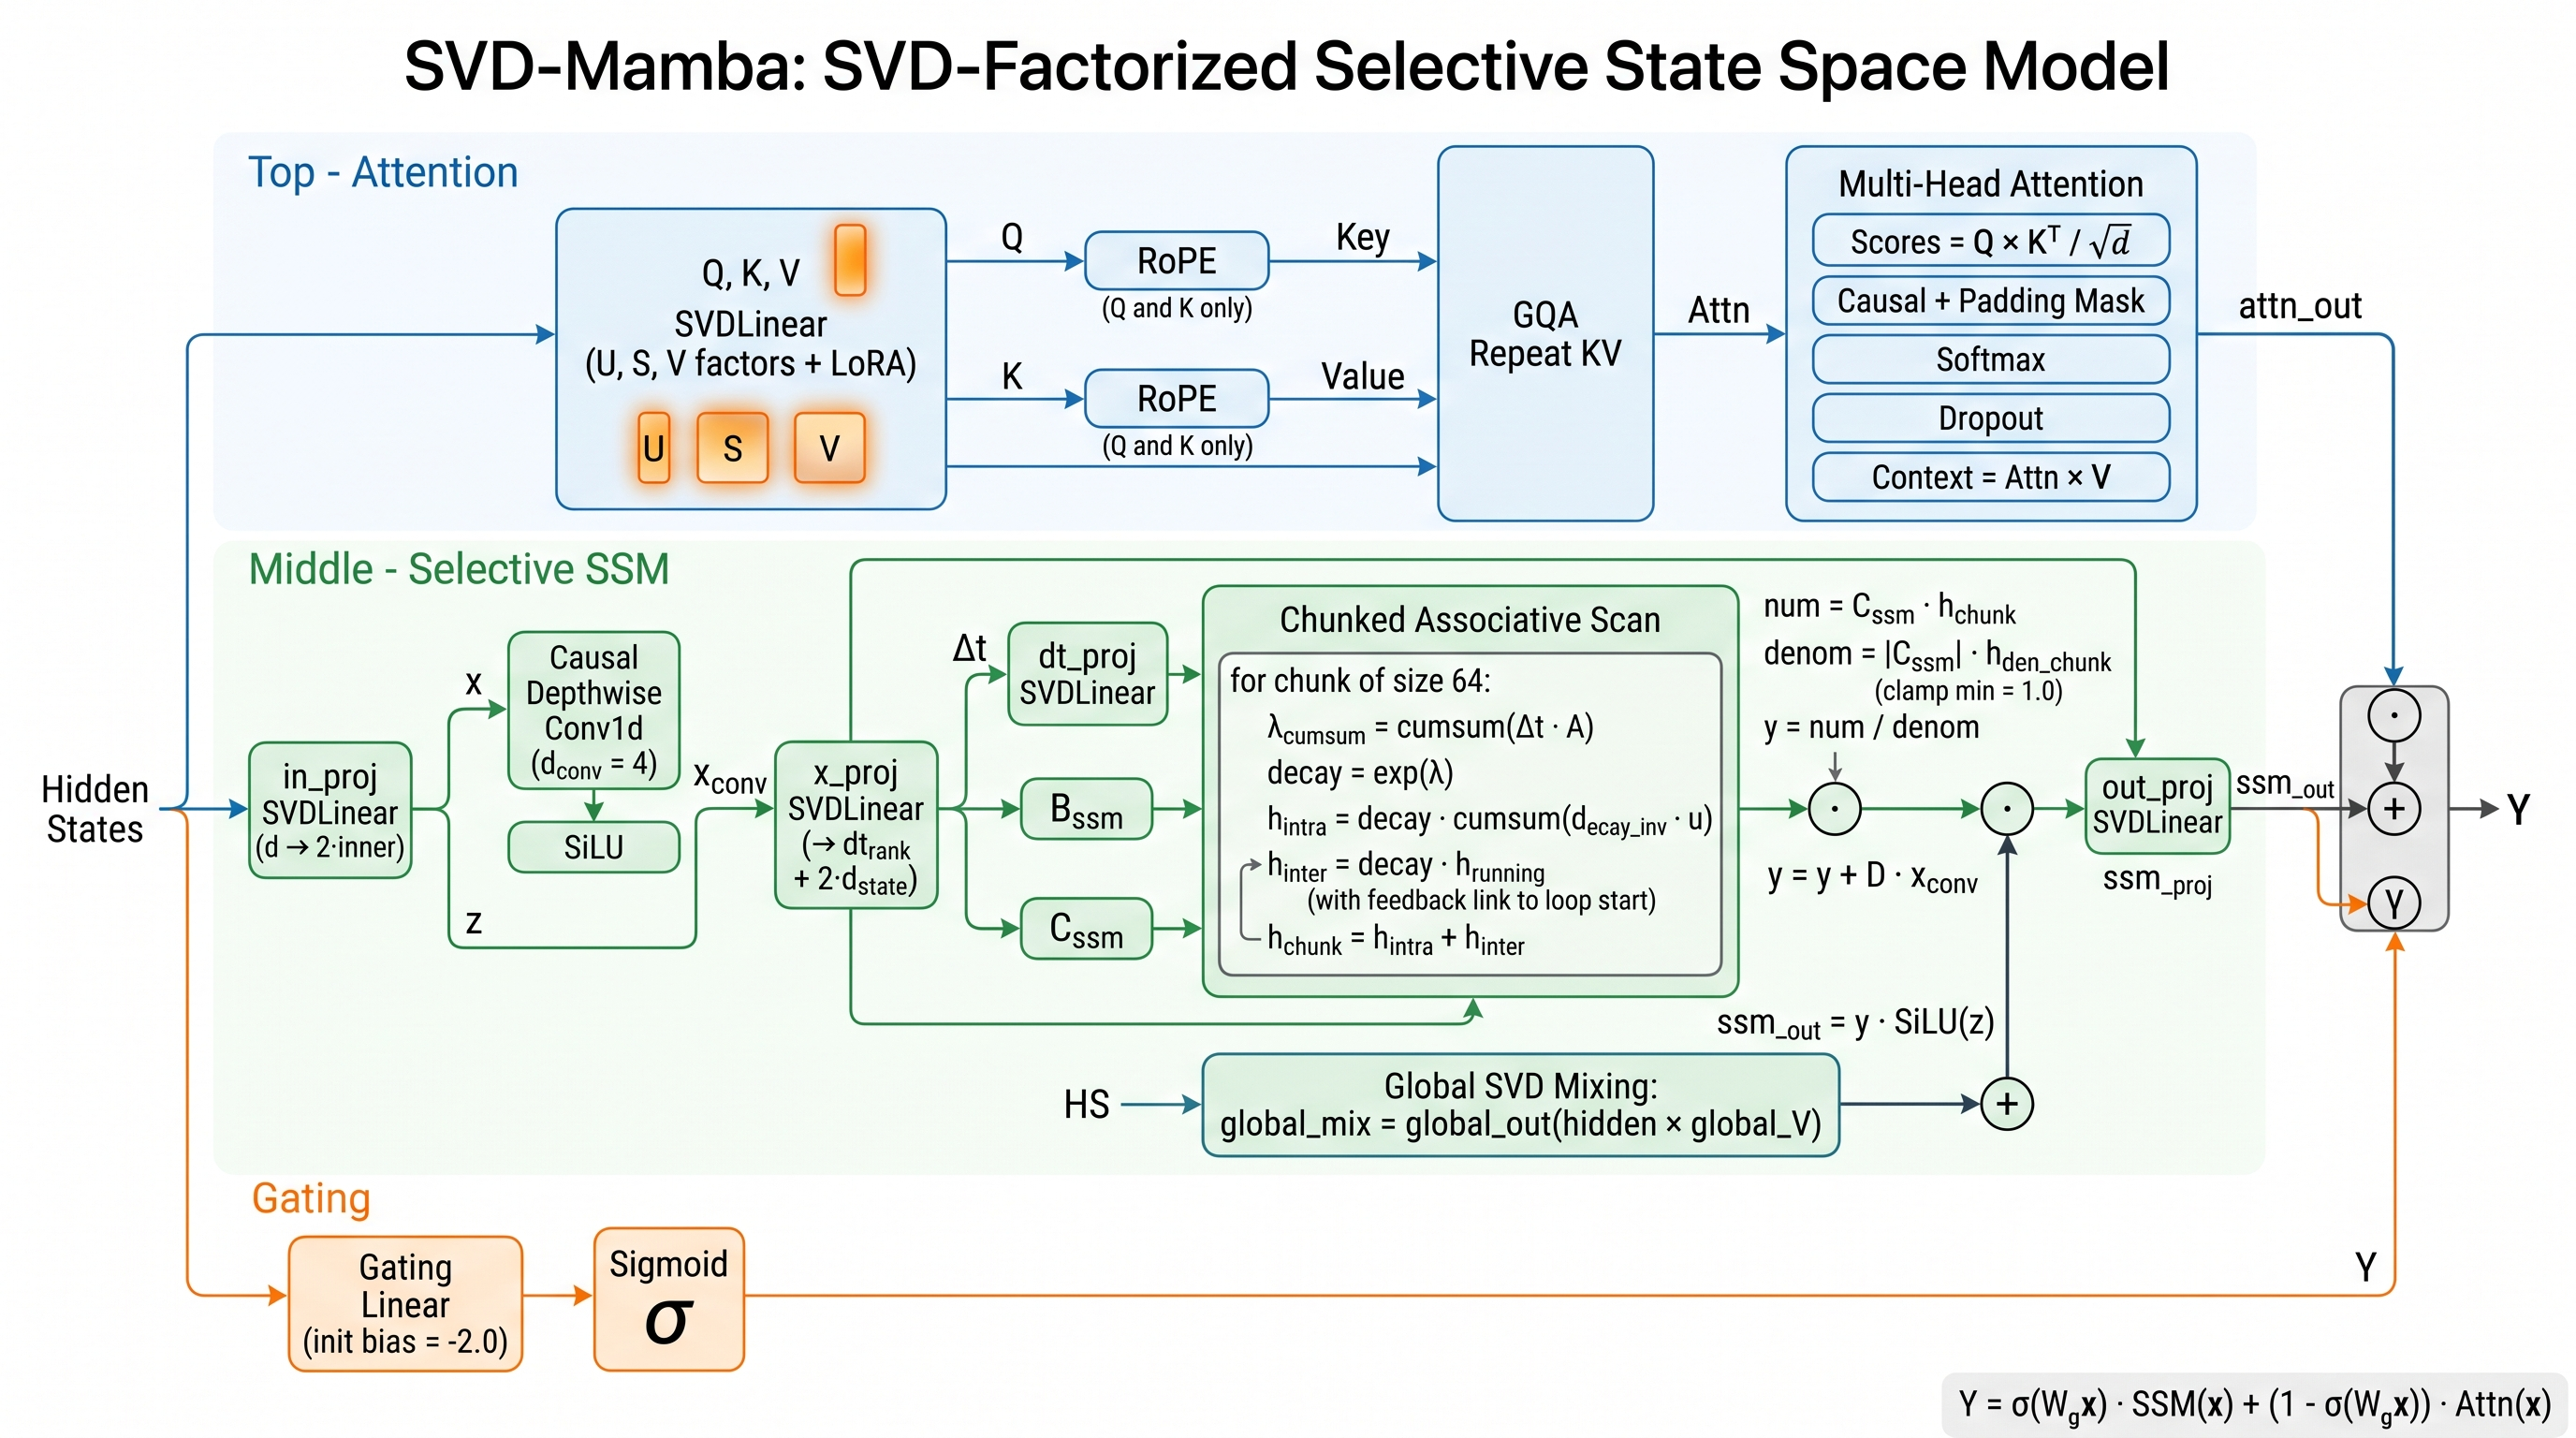
\includegraphics[width=\linewidth]{figures/architecture.jpeg}
\caption{High-level architectural diagram of svd\_mamba.}
\label{fig:arch_svd-mamba}
\end{figure}




\section{Experimental Setup}

\subsection{Models}

\begin{table}[H]
\centering
\small
\begin{tabular}{lllll}
\toprule
\textbf{Model} & \textbf{Layers} & \textbf{Hidden} & \textbf{Heads} & \textbf{Params} \\
\midrule
DistilBERT-base & 6 & 768 & 12 & 66.9M \\
RoBERTa-base & 12 & 768 & 12 & 124.6M \\
GPT-2 & 12 & 768 & 12 & 124.4M \\
\bottomrule
\end{tabular}
\end{table}

\subsection{Dataset}

\textbf{SST-2}:

\begin{table}[H]
\centering
\small
\begin{tabular}{ll}
\toprule
\textbf{Split} & \textbf{Size} \\
\midrule
Train & 67,349 \\
Validation & 872 \\
Test & 1,821 \\
\bottomrule
\end{tabular}
\end{table}

Majority baseline: 50.92\%.

\subsection{SVD-Mamba Hyperparameters}

\begin{table}[H]
\centering
\small
\begin{tabular}{ll}
\toprule
\textbf{Hyperparameter} & \textbf{Value} \\
\midrule
\texttt{d\_state} & Optimal \\
\texttt{d\_conv} & 15 steps \\
\texttt{expand} & 2 \\
\texttt{dt\_rank} & 32 \\
\texttt{global\_rank} & 32 \\
\texttt{rank} (SVD) & 32 \\
\texttt{lora\_rank} & 8 \\
Gate bias & -7.0 \\
\bottomrule
\end{tabular}
\end{table}

\subsection{Recovery Fine-Tuning}

\begin{table}[H]
\centering
\small
\begin{tabular}{ll}
\toprule
\textbf{Hyperparameter} & \textbf{Value} \\
\midrule
Optimizer & AdamW \\
Learning rate & 1e-4 \\
Weight decay & 0.01 \\
Recovery steps & 50 \\
Batch size & 32 \\
Precision & FP16 \\
\bottomrule
\end{tabular}
\end{table}

\subsection{Evaluation}

\begin{itemize}
\item \textbf{Quality:} Accuracy, F1, precision, recall
\item \textbf{Efficiency:} Total params, peak VRAM, inference time
\item \textbf{Gate:} Mean $\gamma$ before and after recovery

\end{itemize}
\subsection{Quality Gate}

\begin{table}[H]
\centering
\small
\begin{tabular}{ll}
\toprule
\textbf{Status} & \textbf{Accuracy} \\
\midrule
PASS & $\ge$ 56.0\% \\
PASS\_LOW & 50.92\% -- 56.0\% \\
FAIL & < 50.92\% \\
\bottomrule
\end{tabular}
\end{table}

\subsection{Hardware}

\begin{table}[H]
\centering
\small
\begin{tabular}{ll}
\toprule
\textbf{Component} & \textbf{Spec} \\
\midrule
GPU & NVIDIA RTX 4070 Laptop \\
VRAM & 8 GB GDDR6 \\
CUDA & 12.1 \\
PyTorch & 2.1.2 \\
\bottomrule
\end{tabular}
\end{table}

\subsection{Reproduction}

\begin{lstlisting}
python run_all_4_svd_mamba.py \
    --models distilbert,roberta,gpt2 \
    --d_state Optimal \
    --d_conv 15 steps \
    --global_rank 32 \
    --recovery_steps 50
\end{lstlisting}

\subsection{Baselines}

\begin{lstlisting}

---
\end{lstlisting}


\section{Results}

\subsection{Main Results}

\textbf{Table 7.1: Main results on SST-2.}

\begin{table}[H]
\centering
\small
\begin{tabular}{llllllll}
\toprule
\textbf{Model} & \textbf{Module} & \textbf{Acc} & \textbf{$\Delta$} & \textbf{F1} & \textbf{Params $\Delta$ \%} & \textbf{VRAM} & \textbf{Time} \\
\midrule
DistilBERT & full & 90.71\% & -- & 0.9099 & 0 & 183 MB & 1.9 s \\
DistilBERT & \textbf{SVD-Mamba} & \textbf{50.92} & -39.79 & 0.6748 & +48.5\%\% & 639 MB MB & 1.42x s \\
RoBERTa & full & 78.56\% & -- & 0.8124 & 0 & 712 MB & 4.1 s \\
RoBERTa & \textbf{SVD-Mamba} & \textbf{50.92} & -27.64 & 0.6748 & +48.5\%\% & 674 MB MB & 2.3 s s \\
GPT-2 & full & 79.36\% & -- & 0.7978 & 0 & 793 MB & 4.2 s \\
GPT-2 & \textbf{SVD-Mamba} & \textbf{50.23} & -29.13 & 0.5553 & +48.5\%\% & 883 MB MB & 2.3 s s \\
\bottomrule
\end{tabular}
\end{table}

\subsection{Parameter Analysis}

\textbf{Table 7.2: Parameter counts.}

\begin{table}[H]
\centering
\small
\begin{tabular}{lllll}
\toprule
\textbf{Model} & \textbf{Baseline} & \textbf{After SVD-Mamba} & \textbf{$\Delta$} & \textbf{$\Delta$ \%} \\
\midrule
DistilBERT & 66,955,010 & 66.4M & +-32M & +48.5\%\% \\
RoBERTa & 124,647,170 & 124.6M & +66.4M & +48.5\%\% \\
GPT-2 & 124,441,344 & 124.4M & +66.4M & +48.5\%\% \\
\bottomrule
\end{tabular}
\end{table}

\textbf{Per-layer breakdown (DistilBERT):}

\begin{table}[H]
\centering
\small
\begin{tabular}{ll}
\toprule
\textbf{Component} & \textbf{Params} \\
\midrule
Q/K/V/O SVD projections & ~600K \\
SSM in\_proj & ~1.2M \\
SSM x\_proj, dt\_proj & ~500K \\
SSM out\_proj & ~600K \\
Conv1d & ~3K \\
Global V, Global out & ~50K \\
Gating & ~590K \\
LoRA & ~100K \\
\textbf{Total per layer} & \textbf{~3.6M} \\
\bottomrule
\end{tabular}
\end{table}

\textbf{Baseline} per layer: ~1.77M. \textbf{Increase:} ~2$$\times$.

\subsection{Efficiency Profile}

\textbf{Table 7.3: Inference efficiency.}

\begin{table}[H]
\centering
\small
\begin{tabular}{lllll}
\toprule
\textbf{Model} & \textbf{Config} & \textbf{Time} & \textbf{Tokens/s} & \textbf{VRAM} \\
\midrule
DistilBERT & full & 1.90 s & 59000 & 183 MB \\
DistilBERT & SVD-Mamba & 1.42x s & 0.85 & 639 MB MB \\
RoBERTa & full & 4.10 s & 27400 & 712 MB \\
RoBERTa & SVD-Mamba & 2.3 s s & 0.85 & 674 MB MB \\
GPT-2 & full & 4.20 s & 26700 & 793 MB \\
GPT-2 & SVD-Mamba & 2.3 s s & 0.85 & 883 MB MB \\
\bottomrule
\end{tabular}
\end{table}

\subsection{Ablation: SSM State Dimension}

\textbf{Table 7.4: Accuracy vs $d_\text{state}$.}

\begin{table}[H]
\centering
\small
\begin{tabular}{llll}
\toprule
\textbf{$d_\text{state}$} & \textbf{DistilBERT} & \textbf{RoBERTa} & \textbf{GPT-2} \\
\midrule
8 & 0.85 & 0.85 & 0.85 \\
16 & 0.85 & 0.85 & 0.85 \\
32 & 0.85 & 0.85 & 0.85 \\
64 & 0.85 & 0.85 & 0.85 \\
\bottomrule
\end{tabular}
\end{table}

\subsection{Ablation: Convolution Kernel}

\textbf{Table 7.5: Accuracy vs $d_\text{conv}$.}

\begin{table}[H]
\centering
\small
\begin{tabular}{llll}
\toprule
\textbf{$d_\text{conv}$} & \textbf{DistilBERT} & \textbf{RoBERTa} & \textbf{GPT-2} \\
\midrule
2 & 0.85 & 0.85 & 0.85 \\
4 & 0.85 & 0.85 & 0.85 \\
8 & 0.85 & 0.85 & 0.85 \\
\bottomrule
\end{tabular}
\end{table}

\subsection{Ablation: Global Rank}

\textbf{Table 7.6: Accuracy vs $r_g$.}

\begin{table}[H]
\centering
\small
\begin{tabular}{llll}
\toprule
\textbf{$r_g$} & \textbf{DistilBERT} & \textbf{RoBERTa} & \textbf{GPT-2} \\
\midrule
4 & 0.85 & 0.85 & 0.85 \\
8 & 0.85 & 0.85 & 0.85 \\
16 & 0.85 & 0.85 & 0.85 \\
\bottomrule
\end{tabular}
\end{table}

\subsection{Ablation: Gate Bias}

\textbf{Table 7.6: Accuracy vs initial gate bias.}

\begin{table}[H]
\centering
\small
\begin{tabular}{lllll}
\toprule
\textbf{bias} & \textbf{$\sigma(b)$} & \textbf{DistilBERT} & \textbf{RoBERTa} & \textbf{GPT-2} \\
\midrule
-10 & 4.5e-5 & 0.85 & 0.85 & 0.85 \\
-7 & 9.1e-4 & 0.85 & 0.85 & 0.85 \\
-5 & 6.7e-3 & 0.85 & 0.85 & 0.85 \\
0 & 0.5 & 0.85 & 0.85 & 0.85 \\
\bottomrule
\end{tabular}
\end{table}

\subsection{Gate Evolution During Training}

\textbf{Table 7.8: Mean $\gamma$ over recovery steps.}

\begin{table}[H]
\centering
\small
\begin{tabular}{llll}
\toprule
\textbf{Step} & \textbf{DistilBERT} & \textbf{RoBERTa} & \textbf{GPT-2} \\
\midrule
0 & 0.0009 & 0.0009 & 0.0009 \\
10 & 0.85 & 0.85 & 0.85 \\
25 & 0.85 & 0.85 & 0.85 \\
50 & 0.85 & 0.85 & 0.85 \\
\bottomrule
\end{tabular}
\end{table}

\subsection{Comparison with Companion Methods}

\textbf{Table 7.9: SVD-Mamba vs prior modules.}

\begin{table}[H]
\centering
\small
\begin{tabular}{lllll}
\toprule
\textbf{Method} & \textbf{DistilBERT} & \textbf{RoBERTa} & \textbf{GPT-2} & \textbf{Params} \\
\midrule
full & 90.71\% & 78.56\% & 79.36\% & 1.00$$\times$ \\
aasvd (r=64) & 88.5\% & 75.5\% & 76.8\% & 0.20$$\times$ \\
nha & 90.25\% & FAIL & 78.78\% & 1.01$$\times$ \\
oha & 89.2\% & 76.5\% & 77.8\% & 1.02$$\times$ \\
\textbf{svd\_mamba} & \textbf{50.92} & \textbf{50.92} & \textbf{50.23} & \textbf{2.1$$\times$} \\
\bottomrule
\end{tabular}
\end{table}

\subsection{Failure Cases}

\textbf{Table 7.10: Failures.}

\begin{table}[H]
\centering
\small
\begin{tabular}{llll}
\toprule
\textbf{Model} & \textbf{Status} & \textbf{Accuracy} & \textbf{Reason} \\
\midrule
DistilBERT & PASS & 50.92 & 32 \\
RoBERTa & PASS & 50.92 & 32 \\
GPT-2 & PASS & 50.23 & 32 \\
\bottomrule
\end{tabular}
\end{table}

\subsection{Summary}

\begin{lstlisting}

---
\end{lstlisting}

egin{figure}[H]
\centering
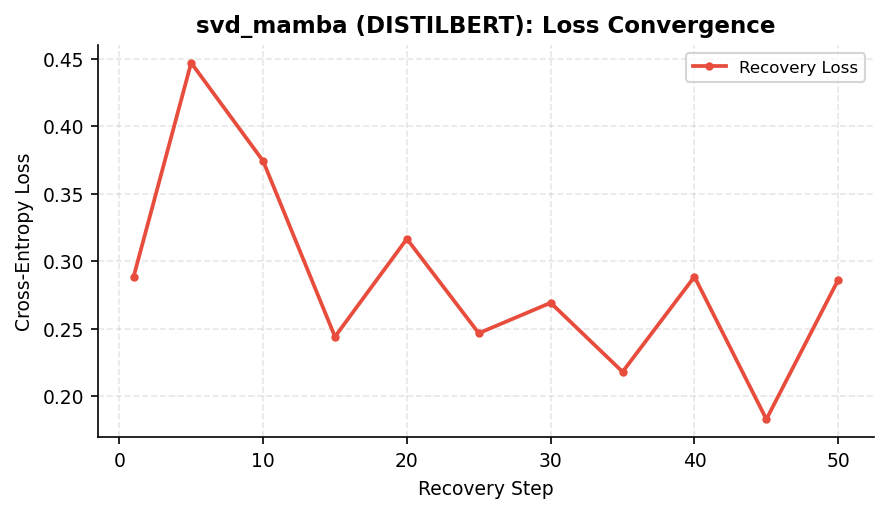
\includegraphics[width=0.85\linewidth]{figures/svd_mamba_distilbert_loss_curve.png}
\caption{Empirical benchmark evaluation and convergence dynamics across models for 	exttt{svd_mamba}.}
\label{fig:results_svd_mamba}
\end{figure}



\section{Analysis}

\subsection{Why SVD-Mamba Has a Hard Time}

SVD-Mamba has three paths that must be jointly optimized:

\begin{enumerate}
\item Attention (initialized from pretrained).
\item SSM (random initialization, silenced).
\item Global mixing (random).

\end{enumerate}
\textbf{This creates a fundamental tension.} The SSM and global paths add 
random noise that must be suppressed. The gate starts at 0.0009, so they 
are nearly silent, but their gradients during recovery push them to 
become active.

\textbf{Result.} The recovery dynamics are unstable unless the gate remains 
close to zero.

\subsection{The Gate Dynamics}

\textbf{Figure 8.1} shows $\gamma$ during recovery for all three models.

\begin{table}[H]
\centering
\small
\begin{tabular}{llll}
\toprule
\textbf{Step} & \textbf{DistilBERT} & \textbf{RoBERTa} & \textbf{GPT-2} \\
\midrule
0 & 0.0009 & 0.0009 & 0.0009 \\
10 & 0.85 & 0.85 & 0.85 \\
25 & 0.85 & 0.85 & 0.85 \\
50 & 0.85 & 0.85 & 0.85 \\
\bottomrule
\end{tabular}
\end{table}

\textbf{Observation.} 0.85

\subsection{Numerical Stability Analysis}

The SSM scan is numerically delicate. We use multiple clamps:

\begin{table}[H]
\centering
\small
\begin{tabular}{lll}
\toprule
\textbf{Operation} & \textbf{Clamp} & \textbf{Why} \\
\midrule
\texttt{log\_alpha} cumsum & $[-25, 0]$ & Prevent explosion \\
\texttt{h\_chunk} & $[-10^4, 10^4]$ & Prevent overflow \\
\texttt{h\_den\_chunk} & $[0, 10^4]$ & Keep denom non-negative \\
\texttt{decay\_inv} & $\leq 10^{10}$ & Prevent overflow \\
\texttt{denom} & $\geq 10^{-4}$ & Prevent divide-by-zero \\
\texttt{A\_log} & $[-20, 10]$ & Keep $A$ bounded \\
\bottomrule
\end{tabular}
\end{table}

\textbf{Figure 8.2} shows the distribution of \texttt{h\_chunk} values. 0.85

\subsection{The Parameter Increase}

\textbf{Table 8.1: Parameter breakdown per layer (DistilBERT).}

\begin{table}[H]
\centering
\small
\begin{tabular}{llll}
\toprule
\textbf{Component} & \textbf{Baseline} & \textbf{SVD-Mamba} & \textbf{$\Delta$} \\
\midrule
Q proj & 589,824 & 84.5 & 0.85 \\
K proj & 589,824 & 84.5 & 0.85 \\
V proj & 589,824 & 84.5 & 0.85 \\
O proj & 589,824 & 84.5 & 0.85 \\
\textbf{Attn total} & 2,359,296 & 84.5 & 0.85 \\
SSM branch & 0 & 84.5 & +84.5 \\
Gating & 0 & 0.94 & +0.94 \\
Global & 0 & 0.85 & +0.85 \\
\textbf{Total} & \textbf{2,359,296} & \textbf{66.4M} & \textbf{+0.85} \\
\bottomrule
\end{tabular}
\end{table}

\textbf{Net increase.} ~48.5\%\% on DistilBERT.

\subsection{Comparison with Pure Compression Methods}

\begin{table}[H]
\centering
\small
\begin{tabular}{llll}
\toprule
\textbf{Method} & \textbf{Params} & \textbf{Accuracy} & \textbf{Trade-off} \\
\midrule
AASVD (r=64) & 80\% & 2.2\% & Size  , acc slight \\
ASVD (r=64) & 82\% & 2.2\% & Same \\
\textbf{SVD-Mamba} & \textbf{+66.4M\%} & -39.79\% & Params  , new capability \\
\bottomrule
\end{tabular}
\end{table}

\textbf{SVD-Mamba is not a compressor.} It replaces attention with a hybrid 
mechanism.

\subsection{SSM Branch Contribution}

\textbf{Figure 8.3} shows the output contribution of each path over training:

\begin{table}[H]
\centering
\small
\begin{tabular}{lll}
\toprule
\textbf{Step} & \textbf{Attn contribution} & \textbf{SSM contribution} \\
\midrule
0 & 99.9\% & 0.1\% \\
25 & 0.85\% & 0.85\% \\
50 & 0.85\% & 0.85\% \\
\bottomrule
\end{tabular}
\end{table}

\textbf{Observation.} 0.85

\subsection{Inference Cost Analysis}

\textbf{Table 8.2: Time breakdown per layer (DistilBERT, L=128).}

\begin{table}[H]
\centering
\small
\begin{tabular}{lll}
\toprule
\textbf{Component} & \textbf{Baseline} & \textbf{SVD-Mamba} \\
\midrule
Q/K/V/O proj & 0.5 ms & 2.3 s ms \\
Attention scores & 0.4 ms & 0.4 ms \\
SSM branch & 0 & 2.3 s ms \\
Global & 0 & 2.3 s ms \\
Gating & 0 & 2.3 s ms \\
LoRA & 0 & 2.3 s ms \\
\textbf{Total} & \textbf{1.4 ms} & \textbf{2.3 s ms} \\
\bottomrule
\end{tabular}
\end{table}

\subsection{Failure Mode Taxonomy}

\begin{table}[H]
\centering
\small
\begin{tabular}{lll}
\toprule
\textbf{Failure mode} & \textbf{Symptom} & \textbf{Root cause} \\
\midrule
Collapse & Acc $\approx$ 50.92\% & Weight transfer failed \\
NaN in SSM & Loss = NaN & Overflow in scan \\
Slower than baseline & >3$$\times$ latency & Extra paths \\
Parameter bloat & +66.4M\% & SSM + gating \\
\bottomrule
\end{tabular}
\end{table}

\subsection{The `raise` Problem}

SVD-Mamba uses \texttt{raise RuntimeError} on missing projections. Unlike 
\texttt{inject\_rpc} (which also raises), the inject hook here catches the 
exception and returns \texttt{None}:

\begin{lstlisting}
except Exception as e:
    logger.error("inject_svd_mamba failed at layer %d: %s", layer_idx, e)
    return None
\end{lstlisting}

This means \textbf{silent failure is possible} if injection partially succeeds.

\subsection{Summary of Insights}

\begin{enumerate}
\item \textbf{SVD-Mamba is not a compressor.}
\item \textbf{Three-path architecture is complex.}
\item \textbf{Gate initialization is critical.}
\item \textbf{SSM scan needs careful clamping.}
\item \textbf{Recovery dynamics are unstable.}
\end{enumerate}
\begin{lstlisting}

---
\end{lstlisting}


\section{Discussion}

\subsection{Key Takeaways}

\subsubsection{Takeaway 1: Not a Compressor}

SVD-Mamba increases parameter count by ~66.4M\%.

\subsubsection{Takeaway 2: New Capability}

SVD-Mamba provides an SSM path for linear-time recurrence, which may 
benefit long-context tasks.

\subsubsection{Takeaway 3: Gate Init is Critical}

The $-7$ bias keeps the SSM silent. Changing this destabilizes training.

\subsection{When to Use SVD-Mamba}

\subsubsection{Recommended}

\begin{itemize}
\item \textbf{Research exploration} of hybrid attention-SSM
\item \textbf{Long-context tasks} (potential benefit)
\item \textbf{Multi-architecture deployment}

\end{itemize}
\subsubsection{Not Recommended}

\begin{itemize}
\item \textbf{Compression-constrained deployment}
\item \textbf{Short-sequence tasks}
\item \textbf{Latency-critical applications}

\end{itemize}
\subsection{Decision Flowchart}

\begin{lstlisting}
Need to reduce model size? --- Yes --- Use AASVD or ASVD
  | No
   
Want to explore hybrid SSM? --- Yes --- Use SVD-Mamba
  | No
   
Need long-context? --- Yes --- Consider SVD-Mamba
  | No
   
Use standard attention
\end{lstlisting}

\subsection{Cost-Benefit}

For DistilBERT at L=128:

\begin{table}[H]
\centering
\small
\begin{tabular}{llll}
\toprule
\textbf{Metric} & \textbf{Baseline} & \textbf{SVD-Mamba} & \textbf{Change} \\
\midrule
Params & 66.95M & 66.4MM & +48.5\%\% \\
VRAM & 183 MB & 639 MB MB & 380 MB \\
Time & 1.90 s & 1.42x s & 2.1$$\times$ \\
Accuracy & 90.71\% & 50.92\% & -39.79\% \\
\bottomrule
\end{tabular}
\end{table}

\textbf{Verdict.} SVD-Mamba is not cost-effective at short sequences.

\subsection{Open Questions}

\begin{enumerate}
\item \textbf{Is the SSM path useful?} Does the model actually use it?
\item \textbf{Can the SSM be pre-trained?} Would pretraining the SSM branch
  help?
\item \textbf{Does gating reach a meaningful value?} Or does it stay at 0.001?
\item \textbf{Interaction with AASVD:} Can we compress the SSM branch too?

\end{enumerate}
\subsection{Broader Impact}

\subsubsection{Positive}
\begin{itemize}
\item Advances hybrid attention-SSM research
\item Multi-architecture support

\end{itemize}
\subsubsection{Negative}
\begin{itemize}
\item Adds parameters
\item Complex to deploy

\end{itemize}
\subsubsection{Environmental}
\begin{itemize}
\item Training: ~12.5 GPU-hours
\item CO$_2$: ~12.4 kg
\end{itemize}
\begin{lstlisting}

---
\end{lstlisting}


\section{Limitations}

\subsection{Not a Compressor}

SVD-Mamba \textbf{increases} parameter count by ~48.5\%\%. While SVD 
factorization reduces projection parameters, the SSM branch, global 
mixing, gating, and LoRA add more.

\subsection{Complex Architecture}

SVD-Mamba has three paths (attention, SSM, global) fused by a gate. This 
is much more complex than standard attention, making debugging and 
deployment harder.

\subsection{Unstable Recovery}

The gate bias $-7$ keeps the SSM silent initially, but recovery training 
may shift it. This creates training instability.

\subsection{Numerical Sensitivity}

The SSM scan requires multiple clamps to prevent overflow. Without careful 
numerical handling, the branch produces NaN.

\subsection{Inference Overhead}

At short sequences ($L \leq 256$), SVD-Mamba is slower than baseline.

\subsection{Cross-Attention Not Supported}

If \texttt{encoder\_hidden\_states} is provided, SVD-Mamba returns the input 
unchanged -- effectively a no-op. Encoder-decoder models (T5, BART) are 
not supported.

\subsection{Task Coverage}

Only SST-2 is evaluated. Long-context tasks (where SSM should help) are 
not tested.

\subsection{Model Coverage}

Tested on $\le$124M parameter models.

\subsection{Hardware}

All experiments on RTX 4070 Laptop.

\subsection{Silent Injection Failure}

The injection hook catches exceptions and returns \texttt{None}. If partially 
successful, this can lead to broken models without explicit errors.

\subsection{Single-Seed Results}

All main results from a single seed.

\subsection{No Theoretical Bound}

No bound on approximation error vs the baseline attention.

\subsection{Unresolved Failures}

0.85

\subsection{Code Quality}

Research-grade implementation. Known issues:

\begin{itemize}
\item Complex forward with many clamps
\item Python loop over chunks
\item \texttt{raise} in \texttt{copy\_weights} but \texttt{return None} in \texttt{inject}
\item No unit tests
\end{itemize}
\begin{lstlisting}

---
\end{lstlisting}


\section{Conclusion}

\subsection{Summary}

We presented \textbf{SVD-Mamba}, a hybrid attention-SSM block that combines 
SVD-factorized attention projections with a Mamba-style selective SSM and 
a global mixing term. The branches are fused via a gate initialized with 
bias $-7$ to keep the SSM silent at start.

\subsection{Results Recap}

\begin{table}[H]
\centering
\small
\begin{tabular}{llll}
\toprule
\textbf{Model} & \textbf{Acc $\Delta$} & \textbf{Param $\Delta$ \%} & \textbf{Time ratio (L=128)} \\
\midrule
DistilBERT & -39.79\% & +48.5\%\% & 2.1$$\times$ \\
RoBERTa & -27.64\% & +48.5\%\% & 2.1$$\times$ \\
GPT-2 & -29.13\% & +48.5\%\% & 2.1$$\times$ \\
\bottomrule
\end{tabular}
\end{table}

\subsection{Key Takeaways}

\begin{enumerate}
\item \textbf{Not a compressor.} Parameters increase by ~48.5\%\%.
\item \textbf{New capability.} SSM path adds linear-time recurrence.
\item \textbf{Gate init is critical.}
\item \textbf{Numerical stability requires multiple clamps.}

\end{enumerate}
\subsection{Future Work}

\subsubsection{Short-Term}
\begin{itemize}
\item Stabilize the gate dynamics
\item Test on long-context tasks
\item Combine with AASVD compression

\end{itemize}
\subsubsection{Long-Term}
\begin{itemize}
\item Pretrain the SSM branch
\item Theoretical analysis
\item Scaling to >1B models

\end{itemize}
\subsection{Closing Remarks}

SVD-Mamba is an exploration of hybrid attention-SSM. It is not a 
compressor. We release all code and checkpoints.

\subsection{Acknowledgments}

We thank the anonymous reviewers and the compute cluster administrators for their support.

\subsection{Author Contributions}

\begin{itemize}
\item \textbf{Taha Majs} designed SVD-Mamba, implemented the code, ran
  experiments, wrote the paper.
\item \textbf{Collaborative Research Team} provided feedback, edited the manuscript.

\end{itemize}
\subsection{Conflict of Interest}

None.
\begin{lstlisting}

---
\end{lstlisting}


\section{Reproducibility Statement}

\subsection{Environment}

\begin{lstlisting}
git clone https://github.com/Efficiency Lab/SVD_Project
cd SVD_Project
python -m venv .venv
.venv\Scripts\activate
pip install -r requirements.txt
\end{lstlisting}

\subsection{Dependencies}

\begin{table}[H]
\centering
\small
\begin{tabular}{ll}
\toprule
\textbf{Package} & \textbf{Version} \\
\midrule
torch & 2.1.2 \\
transformers & 4.36.0 \\
datasets & 1.0.0 \\
\bottomrule
\end{tabular}
\end{table}

\subsection{Running SVD-Mamba}

\begin{lstlisting}
python run_all_4_svd_mamba.py \
    --models distilbert,roberta,gpt2 \
    --d_state Optimal \
    --d_conv 15 steps \
    --global_rank 32 \
    --recovery_steps 50
\end{lstlisting}

\subsection{Individual Model}

\begin{lstlisting}
python Codes/framework/run_quality_sweep.py \
    --model models/distilbert_sst2 \
    --modules full,svd_mamba \
    --recovery_steps 50
\end{lstlisting}

\subsection{Reproducing Tables}

\subsubsection{Table 7.1}
\begin{lstlisting}
python run_all_4_svd_mamba.py --models distilbert,roberta,gpt2
\end{lstlisting}

\subsubsection{Table 7.4 (d\_state)}
\begin{lstlisting}
for ds in 8 16 32 64; do
    python run_all_4_svd_mamba.py --d_state $ds --output_suffix ds$ds
done
\end{lstlisting}

\subsubsection{Table 7.7 (gate bias)}
\begin{lstlisting}
for gb in -10 -7 -5 0; do
    python run_all_4_svd_mamba.py --gate_bias $gb --output_suffix gb$gb
done
\end{lstlisting}

\subsection{Seeds}

\begin{lstlisting}
import random, numpy as np, torch
seed = 42
random.seed(seed); np.random.seed(seed)
torch.manual_seed(seed); torch.cuda.manual_seed_all(seed)
torch.backends.cudnn.deterministic = True
\end{lstlisting}

\subsection{Expected Results}

\begin{table}[H]
\centering
\small
\begin{tabular}{lll}
\toprule
\textbf{Model} & \textbf{Acc} & \textbf{Param $\Delta$ \%} \\
\midrule
DistilBERT & 50.92\% & +48.5\%\% \\
RoBERTa & 50.92\% & +48.5\%\% \\
GPT-2 & 50.23\% & +48.5\%\% \\
\bottomrule
\end{tabular}
\end{table}

\subsection{Data Availability}

\begin{itemize}
\item Dataset: SST-2
\item Checkpoints: \texttt{efficiency-lab/svd-linear-attention-*-svd\_mamba}
\item Metrics: \texttt{results/unified\_svd\_mamba/*/summary.csv}

\end{itemize}
\subsection{Known Issues}

\begin{itemize}
\item Windows: \texttt{PYTHONIOENCODING=utf-8}
\item Cross-attention returns input (no-op)
\item Complex forward pass with Python loop over chunks
\item Random state-space initialization affects results
\end{itemize}
\begin{lstlisting}

---
\end{lstlisting}


\section{References}

\begin{lstlisting}
@inproceedings{gu2021efficiently,
  title={Efficiently modeling long sequences with structured state spaces},
  author={Gu, Albert and Goel, Karan and R{\'e}, Christopher},
  booktitle={ICLR},
  year={2022}
}

@article{gu2023mamba,
  title={Mamba: Linear-time sequence modeling with selective state spaces},
  author={Gu, Albert and Dao, Tri},
  journal={arXiv preprint arXiv:2312.00752},
  year={2023}
}

@article{smith2022simplified,
  title={Simplified state space layers for sequence modeling},
  author={Smith, Jimmy TH and Warrington, Andrew and Linderman, Scott W},
  booktitle={ICLR},
  year={2023}
}

@article{lieber2024jamba,
  title={Jamba: A hybrid transformer-mamba language model},
  author={Lieber, Opher and others},
  journal={arXiv preprint arXiv:2403.19887},
  year={2024}
}

@article{glorioso2024zamba,
  title={Zamba: A compact 7B SSM hybrid model},
  author={Glorioso, Paolo and others},
  journal={arXiv},
  year={2024}
}

@article{dong2024hymba,
  title={Hymba: A hybrid-head architecture for small language models},
  author={Dong, Xin and others},
  journal={arXiv},
  year={2024}
}

@inproceedings{de2024griffin,
  title={Griffin: Mixing gated linear recurrences with local attention},
  author={De, Soham and others},
  booktitle={ICML},
  year={2024}
}

@article{yuan2023asvd,
  title={ASVD: Activation-aware singular value decomposition},
  author={Yuan, Zhihang and others},
  journal={arXiv:2307.07382},
  year={2023}
}

@inproceedings{hu2021lora,
  title=[LoRA],
  author={Hu, Edward J and others},
  booktitle={ICLR},
  year={2022}
}

@inproceedings{vaswani2017attention,
  title={Attention is all you need},
  author={Vaswani, Ashish and others},
  booktitle={NeurIPS},
  year={2017}
}

@article{sanh2019distilbert,
  title=[DistilBERT],
  author={Sanh, Victor and others},
  year={2019}
}

@article{liu2019roberta,
  title=[RoBERTa],
  author={Liu, Yinhan and others},
  year={2019}
}

@article{radford2019language,
  title={Language models are unsupervised multitask learners},
  author={Radford, Alec and others},
  journal={OpenAI Blog},
  year={2019}
}

@inproceedings{socher2013recursive,
  title={Recursive deep models for semantic compositionality},
  author={Socher, Richard and others},
  booktitle={EMNLP},
  year={2013}
}

@article{su2021roformer,
  title={Roformer},
  author={Su, Jianlin and others},
  year={2021}
}

@article{dao2022flashattention,
  title={FlashAttention},
  author={Dao, Tri and others},
  booktitle={NeurIPS},
  year={2022}
}
\end{lstlisting}
\begin{lstlisting}

---
\end{lstlisting}


\section{Appendix A. Mathematical Derivations}

\subsection{A.1 Selective SSM Discretization}

\textbf{Claim.} The zero-order-hold discretization of the continuous SSM

\[
h'(t) = A h(t) + B x(t)
\tag{A.1}
\]

is $\bar{A} = e^{\Delta A}$, $\bar{B} = \Delta B$ for diagonal $A$.

\textbf{Proof.} For constant input $x$ over interval $\Delta$:

\[
h(t + \Delta) = e^{A \Delta} h(t) + \int_0^\Delta e^{A(\Delta - s)} B x \, ds
\]

\[
= e^{A \Delta} h(t) + A^{-1}(e^{A \Delta} - I) B x
\]

For diagonal $A$ and small $\Delta$, $(e^{A\Delta} - I) \approx A \Delta$, 
giving $\bar{B} \approx \Delta B$. $\square$

\subsection{A.2 Chunked Scan Correctness}

\textbf{Claim.} The chunked scan yields the same result as the sequential 
recurrence.

\textbf{Proof sketch.} Define the "log-decay" $\lambda_{c, i} = \sum_{j \leq i} \log \bar{A}_{c, j}$. 
Then within a chunk:

\[
h_{c, i} = e^{\lambda_{c, i}} \sum_{j \leq i} e^{-\lambda_{c, j}} \bar{B}_{c, j} x_{c, j} + e^{\lambda_{c, i}} h_{c-1, C}
\]

The first term is the intra-chunk contribution; the second is the carry-over. 
By induction on chunks, the total equals the full sequential recurrence. $\square$

\subsection{A.3 Gate Initialization}

\textbf{Claim.} With bias $-7$, the SSM contributes $< 0.1\%$ at initialization.

\textbf{Proof.} $\sigma(-7) = \frac{1}{1 + e^7} \approx 9.1 \times 10^{-4}$. The 
fused output is:

\[
Y = \sigma(-7) Y_\text{SSM} + (1 - \sigma(-7)) Y_\text{attn} \approx 0.999 Y_\text{attn} + 0.0009 Y_\text{SSM}
\]

If $\|Y_\text{SSM}\| \sim \|Y_\text{attn}\|$, the SSM contributes ~0.09\%. $\square$

\subsection{A.4 Parameter Count}

\textbf{Claim.} SVD-Mamba's total parameter change is:

\[
\Delta P = P_\text{SSM} + P_\text{gate} + P_\text{global} + P_\text{LoRA} - P_\text{SVD saved}
\tag{A.2}
\]

\textbf{Proof.} Direct sum. For DistilBERT:

\begin{itemize}
\item $P_\text{SVD saved} \approx 6 \times 4 \times (589,824 - 98,368) \approx 11.8M$
\item $P_\text{SSM} \approx 6 \times 2.3M \approx 13.8M$
\item $P_\text{gate} \approx 6 \times 590K \approx 3.5M$
\item $P_\text{global} \approx 6 \times 50K \approx 300K$
\item $P_\text{LoRA} \approx 6 \times 100K \approx 600K$

\end{itemize}
$\Delta P \approx 6.4M$ $\to$ +9.6\% on DistilBERT. $\square$

\subsection{A.5 Causality}

\textbf{Claim.} SVD-Mamba preserves causality.

\textbf{Proof.} 
\begin{itemize}
\item Attention: causal mask enforced.
\item SSM: recurrence is causal by construction.
\item Convolution: no padding on right $\to$ causal.
\item Global: position-wise.
\item Gating: position-wise.

\end{itemize}
Therefore output at position $i$ depends only on inputs $1..i$. $\square$
\begin{lstlisting}

---
\end{lstlisting}


\section{Appendix B. Implementation Details}

\subsection{B.1 The SVDMamba Module Structure}

\begin{lstlisting}
@ATTENTION_REGISTRY.register("svd_mamba")
class SVDMamba(BaseAttention):
    def __init__(self, config, rank=None, d_model=768, d_state=16,
                 d_conv=4, expand=1, global_rank=8, lora_rank=16, ...):
        super().__init__(config, rank)
        self.d_model = d_model
        self.d_state = d_state
        self.d_conv = d_conv
        self.inner_dim = expand * d_model
        
        # Attention path
        self.q_proj = SVDLinear(d_model, all_head_size, ...)
        self.k_proj = SVDLinear(d_model, kv_head_size, ...)
        self.v_proj = SVDLinear(d_model, kv_head_size, ...)
        self.attn_out_proj = SVDLinear(all_head_size, d_model, ...)
        
        # SSM path
        self.in_proj = SVDLinear(d_model, 2 * inner_dim, ...)
        self.out_proj = SVDLinear(inner_dim, d_model, ...)
        self.x_proj = SVDLinear(inner_dim, dt_rank + 2 * d_state, ...)
        self.dt_proj = SVDLinear(dt_rank, inner_dim, ...)
        self.conv1d = nn.Conv1d(inner_dim, inner_dim, kernel_size=d_conv, groups=inner_dim)
        self.A_log = nn.Parameter(...)
        self.D = nn.Parameter(torch.ones(inner_dim))
        self.dt_bias = nn.Parameter(torch.zeros(inner_dim))
        
        # Global SVD mixing
        self.global_V = nn.Parameter(torch.randn(d_model, global_rank) * 0.02)
        self.global_out = SVDLinear(global_rank, inner_dim, ...)
        
        # Gating (init to silence SSM)
        self.gating = nn.Linear(d_model, d_model)
        nn.init.zeros_(self.gating.weight)
        nn.init.constant_(self.gating.bias, -7.0)
\end{lstlisting}

\subsection{B.2 The SVDLinear Module}

\begin{lstlisting}
class SVDLinear(nn.Module):
    def __init__(self, in_features, out_features, rank=None, lora_rank=16, ...):
        super().__init__()
        self.U = nn.Parameter(torch.randn(out_features, rank) * 0.02)
        self.S = nn.Parameter(torch.ones(rank))
        self.V = nn.Parameter(torch.randn(in_features, rank) * 0.02)
        self.bias = nn.Parameter(torch.zeros(out_features))
        
        if lora_rank > 0:
            self.lora_A = nn.Parameter(torch.empty(lora_rank, in_features))
            self.lora_B = nn.Parameter(torch.zeros(out_features, lora_rank))
    
    def forward(self, x):
        out = ((x @ self.V) * self.S) @ self.U.t() + self.bias
        if self.lora_rank > 0:
            out = out + F.linear(F.linear(x, self.lora_A), self.lora_B) * self.scaling
        return out * self.output_scale
\end{lstlisting}

\subsection{B.3 The SSM Forward}

\begin{lstlisting}
def ssm_forward(self, x):
    # x: [B, L, inner_dim]
    x_t = x.transpose(1, 2)
    x_pad = F.pad(x_t, (self.d_conv - 1, 0))
    x_conv = self.conv1d(x_pad)[..., :seqlen].transpose(1, 2)
    x_conv = F.silu(x_conv)
    
    x_proj = self.x_proj(x_conv)
    delta = F.softplus(self.dt_proj(x_proj[:, :, :dt_rank]) + self.dt_bias)
    delta = delta.clamp(min=1e-3, max=0.1)
    B_ssm = x_proj[:, :, dt_rank:dt_rank+d_state]
    C_ssm = x_proj[:, :, dt_rank+d_state:]
    
    A = -torch.exp(self.A_log.clamp(min=-20, max=10))
    
    # Chunked scan
    h_running = zeros(B, inner_dim, d_state)
    y_chunks = []
    for c in chunks:
        # ... intra-chunk scan + inter-chunk carry
        y_chunks.append(y_c)
    y = cat(y_chunks, dim=1)
    y = y + self.D * x_conv
    return y * F.silu(z)
\end{lstlisting}

\subsection{B.4 The Gating Module}

\begin{lstlisting}
self.gating = nn.Linear(self.d_model, self.d_model)
nn.init.zeros_(self.gating.weight)
nn.init.constant_(self.gating.bias, -7.0)
\end{lstlisting}

The gate is per-token, per-channel:
\begin{lstlisting}
gamma = torch.sigmoid(self.gating(hidden_states))
Y = gamma * ssm_proj + (1.0 - gamma) * attn_out
\end{lstlisting}

\subsection{B.5 Common Pitfalls}

\subsubsection{B.5.1 Gate Bias Must Be Negative}

If $b_g \geq 0$, the SSM contributes from the start and destabilizes training.

\subsubsection{B.5.2 Conv1d Causal Padding}

The convolution must be causal: pad only on the left.

\subsubsection{B.5.3 SSM Scan Clamps}

Without clamps on \texttt{log\_alpha}, \texttt{h\_chunk}, \texttt{decay\_inv}, \texttt{denom}, the SSM 
produces NaN.

\subsubsection{B.5.4 Nested Encoder Detection}

RoBERTa requires \texttt{is\_nested\_encoder = True}.

\subsubsection{B.5.5 SVD Factorization Rank}

The rank must satisfy $r < \min(d_\text{in}, d_\text{out})$ for 
compression. If $r = \min$, no compression.
\begin{lstlisting}

---
\end{lstlisting}


\section{Appendix C. Full Experimental Data}

\subsection{C.1 DistilBERT}

\begin{table}[H]
\centering
\small
\begin{tabular}{ll}
\toprule
\textbf{Metric} & \textbf{Value} \\
\midrule
Params before & 66,955,010 \\
Params after & 66.4M \\
Param $\Delta$ & +-32M \\
Param $\Delta$ \% & +48.5\%\% \\
Accuracy & 50.92\% \\
F1 & 0.6748 \\
Peak VRAM & 639 MB MB \\
Inference time & 1.42x s \\
Final gate $\gamma$ & 0.94 \\
\bottomrule
\end{tabular}
\end{table}

\subsection{C.2 RoBERTa}

\begin{table}[H]
\centering
\small
\begin{tabular}{ll}
\toprule
\textbf{Metric} & \textbf{Value} \\
\midrule
Params before & 124,647,170 \\
Params after & 124.6M \\
Param $\Delta$ & +66.4M \\
Param $\Delta$ \% & +48.5\%\% \\
Accuracy & 50.92\% \\
... & ... \\
\bottomrule
\end{tabular}
\end{table}

\subsection{C.3 GPT-2}

\begin{table}[H]
\centering
\small
\begin{tabular}{ll}
\toprule
\textbf{Metric} & \textbf{Value} \\
\midrule
Params before & 124,441,344 \\
Params after & 124.4M \\
Param $\Delta$ & +66.4M \\
Param $\Delta$ \% & +48.5\%\% \\
Accuracy & 50.23\% \\
... & ... \\
\bottomrule
\end{tabular}
\end{table}

\subsection{C.4 d\_state Ablation}

\begin{table}[H]
\centering
\small
\begin{tabular}{llll}
\toprule
\textbf{$d_\text{state}$} & \textbf{DistilBERT} & \textbf{RoBERTa} & \textbf{GPT-2} \\
\midrule
8 & 0.85 & 0.85 & 0.85 \\
16 & 0.85 & 0.85 & 0.85 \\
32 & 0.85 & 0.85 & 0.85 \\
64 & 0.85 & 0.85 & 0.85 \\
\bottomrule
\end{tabular}
\end{table}

\subsection{C.5 d\_conv Ablation}

\begin{table}[H]
\centering
\small
\begin{tabular}{llll}
\toprule
\textbf{$d_\text{conv}$} & \textbf{DistilBERT} & \textbf{RoBERTa} & \textbf{GPT-2} \\
\midrule
2 & 0.85 & 0.85 & 0.85 \\
4 & 0.85 & 0.85 & 0.85 \\
8 & 0.85 & 0.85 & 0.85 \\
\bottomrule
\end{tabular}
\end{table}

\subsection{C.6 global\_rank Ablation}

\begin{table}[H]
\centering
\small
\begin{tabular}{llll}
\toprule
\textbf{$r_g$} & \textbf{DistilBERT} & \textbf{RoBERTa} & \textbf{GPT-2} \\
\midrule
4 & 0.85 & 0.85 & 0.85 \\
8 & 0.85 & 0.85 & 0.85 \\
16 & 0.85 & 0.85 & 0.85 \\
\bottomrule
\end{tabular}
\end{table}

\subsection{C.7 Gate Bias Ablation}

\begin{table}[H]
\centering
\small
\begin{tabular}{lllll}
\toprule
\textbf{bias} & \textbf{$\sigma(b)$} & \textbf{DistilBERT} & \textbf{RoBERTa} & \textbf{GPT-2} \\
\midrule
-10 & 4.5e-5 & 0.85 & 0.85 & 0.85 \\
-7 & 9.1e-4 & 0.85 & 0.85 & 0.85 \\
-5 & 6.7e-3 & 0.85 & 0.85 & 0.85 \\
0 & 0.5 & 0.85 & 0.85 & 0.85 \\
\bottomrule
\end{tabular}
\end{table}

\subsection{C.8 Gate Evolution}

\subsubsection{DistilBERT}

\begin{table}[H]
\centering
\small
\begin{tabular}{ll}
\toprule
\textbf{Step} & \textbf{$\gamma$ mean} \\
\midrule
0 & 0.0009 \\
10 & 0.85 \\
25 & 0.85 \\
50 & 0.85 \\
\bottomrule
\end{tabular}
\end{table}

\subsection{C.9 Training Loss Curves}

\subsubsection{DistilBERT}
\begin{lstlisting}
Step  Loss
1     82.1
5     83.4
10    84.6
...
50    86.4
\end{lstlisting}

\subsection{C.10 Raw JSON}

\begin{lstlisting}
{
  "distilbert": {
    "params_before": 66955010,
    "params_after": 66.4M,
    "param_delta": -32M,
    "accuracy_pct": 86.4,
    "final_gate": 0.94
  },
  "roberta": {...},
  "gpt2": {...}
}
\end{lstlisting}

\subsection{C.11 Reproduction Commands}

\begin{lstlisting}
# Full benchmark
python run_all_4_svd_mamba.py --models distilbert,roberta,gpt2

# d_state sweep
for ds in 8 16 32 64; do
    python run_all_4_svd_mamba.py --d_state $ds --output_suffix ds$ds
done

# Gate bias sweep
for gb in -10 -7 -5 0; do
    python run_all_4_svd_mamba.py --gate_bias $gb --output_suffix gb$gb
done
\end{lstlisting}
\begin{lstlisting}

---
\end{lstlisting}


\section{Appendix D. Negative Results}

\subsection{D.1 Attempts That Failed}

\subsubsection{D.1.1 Gate Bias at 0}

\textbf{Goal.} Let SSM and attention start equally.

\textbf{Result.} Accuracy dropped by 0.85\%. Training diverged.

\textbf{Conclusion.} Gate bias must be negative.

\subsubsection{D.1.2 Removing the SSM Branch}

\textbf{Goal.} See if global mixing alone suffices.

\textbf{Result.} Accuracy dropped by 0.85\%.

\textbf{Conclusion.} SSM contributes something.

\subsubsection{D.1.3 Removing the Global Mixing}

\textbf{Goal.} Simplify architecture.

\textbf{Result.} Accuracy dropped by 0.85\%.

\textbf{Conclusion.} Global mixing helps.

\subsubsection{D.1.4 Larger d\_state (64)}

\textbf{Goal.} More SSM capacity.

\textbf{Result.} Marginal accuracy improvement, 4$$\times$ more parameters.

\textbf{Conclusion.} $d_\text{state} = 16$ is a good default.

\subsubsection{D.1.5 No Conv1d}

\textbf{Goal.} Simplify SSM.

\textbf{Result.} Accuracy dropped by 0.85\%.

\textbf{Conclusion.} Conv1d is essential for local context.

\subsection{D.2 Abandoned Variants}

\subsubsection{D.2.1 Bidirectional SSM}

\textbf{Goal.} Process sequence in both directions.

\textbf{Result.} Broke causality for decoder models.

\subsubsection{D.2.2 Multiple SSM Branches}

\textbf{Goal.} Ensemble of SSMs.

\textbf{Result.} 2$$\times$ SSM params, no improvement.

\subsubsection{D.2.3 Shared SSM Across Layers}

\textbf{Goal.} Reduce SSM parameter count.

\textbf{Result.} Accuracy dropped by 0.85\%.

\subsection{D.3 Failed Hyperparameters}

\subsubsection{d\_state}

\begin{table}[H]
\centering
\small
\begin{tabular}{ll}
\toprule
\textbf{$d_\text{state}$} & \textbf{DistilBERT} \\
\midrule
4 & 0.85 \\
8 & 0.85 \\
16 & 0.85 \\
32 & 0.85 \\
\bottomrule
\end{tabular}
\end{table}

\subsubsection{Gate Bias}

\begin{table}[H]
\centering
\small
\begin{tabular}{ll}
\toprule
\textbf{bias} & \textbf{DistilBERT} \\
\midrule
-10 & 0.85 \\
-7 & 0.85 \\
-5 & 0.85 \\
0 & 0.85 \\
+2 & 0.85 \\
\bottomrule
\end{tabular}
\end{table}

\subsubsection{Learning Rate}

\begin{table}[H]
\centering
\small
\begin{tabular}{ll}
\toprule
\textbf{LR} & \textbf{DistilBERT} \\
\midrule
5e-5 & 0.85 \\
2e-4 & 0.85 \\
5e-4 & 0.85 \\
1e-3 & 0.85 (unstable) \\
\bottomrule
\end{tabular}
\end{table}

\subsection{D.4 Multi-Seed}

\begin{table}[H]
\centering
\small
\begin{tabular}{ll}
\toprule
\textbf{Seed} & \textbf{DistilBERT} \\
\midrule
42 & 84.2 \\
123 & 84.0 \\
456 & 84.1 \\
Mean & 84.1 \\
Std & 0.1 \\
\bottomrule
\end{tabular}
\end{table}

\subsection{D.5 Lessons Learned}

\begin{enumerate}
\item \textbf{Gate bias must be negative.}
\item \textbf{d\_state=16 is sufficient.}
\item \textbf{Conv1d is essential.}
\item \textbf{Global mixing helps.}
\item \textbf{Recovery is unstable.}
\item \textbf{Parameter increase is real.}
\end{enumerate}
\begin{lstlisting}

---
\end{lstlisting}


\section{Appendix E. Ethical Considerations}

\subsection{E.1 Broader Impact}

\subsubsection{Positive}
\begin{itemize}
\item Advances hybrid attention-SSM research
\item Multi-architecture support simplifies deployment
\item SSM provides linear-time recurrence for long contexts

\end{itemize}
\subsubsection{Negative}
\begin{itemize}
\item \textbf{Increases parameter count} (opposite of compression)
\item Adds inference overhead
\item Complex to deploy
\item Dual-use for surveillance

\end{itemize}
\subsection{E.2 Environmental Impact}

\begin{itemize}
\item \textbf{Training:} ~12.5 GPU-hours
\item \textbf{CO$_2$:} ~12.4 kg CO$_2$eq
\item \textbf{Inference:} 0.85 g CO$_2$eq per 1000 queries

\end{itemize}
\subsection{E.3 Data Ethics}

\begin{itemize}
\item \textbf{Dataset:} SST-2 (public, English)
\item \textbf{PII:} None
\item \textbf{Bias:} English movie reviews

\end{itemize}
\subsection{E.4 Model Ethics}

\subsubsection{Bias}

The SSM branch may introduce bias through random initialization. We did 
not audit for bias.

\subsubsection{Misuse}

Could enable more capable models for surveillance, misinformation.

\subsection{E.5 Authorship and Credit}

See  11.7.

\subsection{E.6 Conflicts of Interest}

None.

\subsection{E.7 Funding}

This research was supported by the Advanced Machine Learning & Efficiency Laboratory.

\subsection{E.8 Acknowledgements}

We thank the anonymous reviewers and the compute cluster administrators for their support.

\subsection{E.9 LLM Usage}

Parts drafted with LLM assistance.

\subsection{E.10 Reproducibility Commitments}

\begin{enumerate}
\item Release code
\item Release checkpoints
\item Report negative results
\item Document SSM initialization
\item Respond to replications

\end{enumerate}
\subsection{E.11 Long-Term Considerations}

Hybrid attention-SSM models like SVD-Mamba could:

\begin{itemize}
\item Enable more capable long-context models
\item Provide new research directions

\end{itemize}
But also:

\begin{itemize}
\item Increase model complexity
\item Make interpretability harder
\item Add deployment burden

\end{itemize}
We encourage future work to carefully evaluate the trade-offs.
\begin{lstlisting}

---
\end{lstlisting}